\documentclass[11pt]{amsart}
\pdfinfoomitdate=1
\pdfsuppressptexinfo=-1
\pdftrailerid{}
\usepackage[T1]{fontenc}
\usepackage{lmodern}
\usepackage{mathtools,amssymb,graphicx,booktabs,enumitem,array}
\usepackage[hidelinks]{hyperref}
\hypersetup{
  pdftitle={Closing All Four Open Arithmetic Frontiers: Cubic Lame Non-Congruence, Level (4) Full Congruence on Q(sqrt(33)), Complete 9-Curve Genus-25 Brandt Spectra, and Degree-8 Explicit-Formula Closure},
  pdfauthor={Ergentics},
  pdfkeywords={Nauru graph, dicyclic group Dic6, cubic Lame Shimura curve, Q(sqrt(33)) congruence Shimura curve, Riehm theorem, Brandt matrix, ultra-Ramanujan graph, Poitou-Odlyzko explicit formula, hardware FENV interval arithmetic, Lean 4}
}
\pdfinfo{/Producer () /Creator ()}
\usepackage{microtype}
\numberwithin{equation}{section}
\theoremstyle{plain}
\newtheorem{theorem}{Theorem}[section]
\newtheorem{proposition}[theorem]{Proposition}
\newtheorem{lemma}[theorem]{Lemma}
\newtheorem{corollary}[theorem]{Corollary}
\theoremstyle{definition}\newtheorem{definition}[theorem]{Definition}
\theoremstyle{remark}\newtheorem{remark}[theorem]{Remark}
\newcommand{\Q}{\mathbb{Q}}
\newcommand{\R}{\mathbb{R}}
\newcommand{\C}{\mathbb{C}}
\newcommand{\Z}{\mathbb{Z}}
\newcommand{\F}{\mathbb{F}}
\newcommand{\calO}{\mathcal{O}}
\newcommand{\calE}{\mathcal{E}}
\newcommand{\calC}{\mathcal{C}}
\newcommand{\frP}{\mathfrak{P}}
\newcommand{\frp}{\mathfrak{p}}
\newcommand{\frq}{\mathfrak{q}}
\newcommand{\PGL}{\mathrm{PGL}}
\newcommand{\PSL}{\mathrm{PSL}}
\newcommand{\SL}{\mathrm{SL}}
\newcommand{\GL}{\mathrm{GL}}
\newcommand{\Aut}{\mathrm{Aut}}
\newcommand{\Cay}{\mathrm{Cay}}
\newcommand{\GP}{\mathrm{GP}}
\newcommand{\Dic}{\mathrm{Dic}}
\newcommand{\Stab}{\mathrm{Stab}}
\newcommand{\Ad}{\mathrm{Ad}}
\newcommand{\Ram}{\mathrm{Ram}}
\newcommand{\nrd}{\operatorname{nrd}}
\newcommand{\trd}{\operatorname{trd}}
\newcommand{\ctag}[1]{\textup{\textsf{\scriptsize[#1]}}}
\emergencystretch=4em\hbadness=10000
\raggedbottom

\title[Closing All Four Open Arithmetic Frontiers]{Closing All Four Open Arithmetic Frontiers: Cubic Lam\'e Non-Congruence, Level \texorpdfstring{$(4)$}{(4)} Full Congruence on \texorpdfstring{$\Q(\sqrt{33})$}{Q(sqrt(33))}, Complete $9$-Curve Genus-$25$ Brandt Spectra, and Degree-$8$ Explicit-Formula Closure}
\author{Ergentics}
\date{November 2026}
\subjclass[2020]{Primary 11G18, 14G22, 05C50; Secondary 11R42, 11R52, 20E08}
\keywords{Nauru graph, dicyclic group $\Dic_6$, cubic Lam\'e Shimura curve, $\Q(\sqrt{33})$ congruence Shimura curve, Riehm's theorem, Brandt matrix, ultra-Ramanujan graph, Poitou--Odlyzko explicit formula, IEEE-754 interval arithmetic, Lean~4}

\begin{document}
\begin{abstract}
We resolve all four remaining open arithmetic frontiers left by Paper~\#01 (\emph{Prime Cadences} \cite{ergentics2026pc}), Paper~\#08 / \texttt{PC-II} \cite{ergentics2026pc2}, and Paper~\#09 / \texttt{PC-III} \cite{ergentics2026pc3}, backed by four independent zero-shared-data continuous-integration verification planes (pure Python, zero-crate Rust, dual-compiler freestanding zero-heap hardware-\texttt{FENV} C++20, and live kernel-compiled zero-Mathlib Lean~4.36.0 \cite{mouraullrich2021}).
First (\textbf{Frontier~1}), we prove unconditional non-congruence ($0/8$ realizations) for all four totally real cubic Lam\'e Nauru curves ($d_F \in \{316, 148\}$): both fields are monogenic ($\calO_F = \Z[z]$ with $z=1/x$), prime $3$ is completely inert ($N((3))=27$), explicit $3$-adic square roots of $1-3z$ mod~$81$ isolate unique finite ramification $\Ram_{\mathrm{fin}}(B_{316})=\{v_2\}$ ($N=2$) and $\Ram_{\mathrm{fin}}(B_{148})=\{\frp_5\}$ ($N=5$), universal rank-$12$ maximal orders achieve exact Gram ratios $4=2^2$ and $25=5^2$, Euler-product-verified $|\zeta_F(-1)| \in \{4/3, 1/3\}$ force identical Eichler--Tamagawa mass $M_{\max}=1/3$ ($[\calO^1:\Delta^1]=1$), and local ramified quotients ($C_3$ of $3$-part $3 < 9$ and $C_6$ of order $6 < 36$) unconditionally block $\rho(\Delta^1)$ of order $36$.
Second (\textbf{Frontier~2}), we discover the \textbf{first genuine congruence Shimura curves uniformizing the $3$-adic dicyclic graph $Z = \Cay(\Dic_6, \{x, x^{-1}, y, y^3\})$}: over $F = \Q(\sqrt{33})$ (where $(2)=v_1 v_2$ splits, $\Ram_{\mathrm{fin}}=\varnothing$, $\zeta_F(-1)=1$, $M_{\max}=1/2$), local-global glued rank-$8$ maximal orders $\calO_{33,A}^{\max}$ and exact twin $\calO_{33,B}^{\max}$ ($(u,v)\mapsto(1-u,1-v)$) achieve \textbf{full principal level-$(4)$ congruence} on $4/16$ surjections each ($|L_{\mathrm{signed}}|=2{,}304$, $|L_{\mathrm{proj}}|=1{,}152 = 24\times 48$, $[\pi_1(Z):\Gamma(4)]=48$, $\ker_1=\{1{:}4, 2{:}4, 3{:}4, 6{:}4\}$). We also prove why the modular adjoint $\Ad_{(4)}$ stalls at $|\ker|=2$ via the central mod-$4$ split-prime sign-flip $\sigma = 1 - 2w$ ($\sigma^2 \equiv 1 \pmod 4$, $\sigma \not\equiv \pm 1$), and close all six remaining real-quadratic moduli ($\Q(\sqrt{6})_{A,B}$, $\Q(\sqrt{3})_{A,B}$, and $\Q(\sqrt{13})_{A,B}$ via Riehm's theorem \cite{riehm1970} $\calO_{(2)}^1/[\calO_{(2)}^1,\calO_{(2)}^1]\cong C_5$, $\gcd(4,5)=1$) for an exact census of $8/128$ congruence realizations.
Third (\textbf{Frontier~3}), we compute from first principles all $9/9$ exact $12\times 12$ Hecke Brandt matrices $B(3)$ across the complete torsion-free genus-$25$ Borel Shimura census ($7$ class-number-$1$ curves via prime-power CRT embeddings plus higher-class-number $X_0^{57}(7)$ and $X_0^{1110}(1)$ via HNF/Fincke--Pohst BFS): $0/9$ realize $Z$, the Simple-Graph Trace Gate $\operatorname{tr}(B^2)=48$ rules out $8/9$ multi-edge curves ($\operatorname{tr}(B^2)\in\{52,\dots,68\}$), and the sole simple curve $X_0^{21}(16)$ satisfies $(B-4I)(B-2I)B(B+2I)=0$ with ultra-Ramanujan spectrum $\{4^1, 2^3, 0^3, (-2)^5\}$ ($\lambda_{\mathrm{nt}}=2.0 < 2\sqrt{3}$) and $\operatorname{tr}(B^4)=384 \ne 456$.
Fourth (\textbf{Frontier~4}), we close the degree-$8$ $(8,1,1,E)$ Poitou--Odlyzko explicit-formula window under strict Bochner positivity $f_1(t)=1+\cos(\pi t)\ge 0$ and hardware-\texttt{FENV} certification: eliminating all $7/7$ prime norms $q \le 9$ at $b=3.20$, bounding $c_{11}, c_{13} \le 1$, collapsing local splitting to exactly $5$ $2$-adic and $4$ $3$-adic types, eliminating every nontrivial automorphism ($\mathrm{UB}_{\mathrm{sym}_2} = 12.404760 < 12.595576$, gap $\ge +0.190816$), every nonempty $\Ram_{\mathrm{fin}}$ ($\mathrm{UB}_{\mathrm{Ram}} \le 8.818792$), and every nontrivial Eichler level ($\mathrm{UB}_{\mathrm{Eichler}} \le 10.684210$), isolating the rigid asymmetric free core $d_F \in [633{,}448{,}978;\; 890{,}007{,}374]$ with $|\zeta_F(-1)|=1536$.
\end{abstract}
\maketitle

\section{Introduction and Summary of Main Results}\label{sec:intro}
The Morpheus arithmetic-graph program has traced $p$-adic Mumford uniformization \cite{drinfeld1976,serre1980}, definite and indefinite quaternion Shimura curves \cite{eichler1955,shimura1967,vigneras1980,voight2021}, and Ramanujan expander spectra \cite{lps1988,pizer1980} from the $24$-vertex cubic Tonnetz $X$ (Paper~\#01 \cite{ergentics2026pc}) through the $144$-automorphism bipartite Nauru graph $Y = \GP(12,5)$ (Paper~\#08 / \texttt{PC-II} \cite{ergentics2026pc2}) and its $4$-regular $3$-adic dicyclic companion $Z = \Cay(\Dic_6, \{x, x^{-1}, y, y^3\})$ (Paper~\#09 / \texttt{PC-III} \cite{ergentics2026pc3}).
At the close of \texttt{PC-III} (\texttt{v0.8.0}), exactly four arithmetic frontiers remained open:
\begin{enumerate}[label=(\arabic*),nosep]
\item \textbf{Frontier~1 (Cubic Lam\'e Nauru Moduli):} Determining the finite ramification sets, maximal rank-$12$ orders, exact Eichler--Tamagawa masses, and congruence status of all four irreducible totally real cubic Lam\'e Nauru curves ($d_F \in \{316, 148\}$).
\item \textbf{Frontier~2 (Real-Quadratic $3$-Adic $\Dic_6$ Congruence):} Following the universal $0/80$ rational non-congruence of $Z$ over $\Q$, classifying all primitive real-quadratic Fricke--Vogt moduli $B_Z(u,v)$ and determining whether any split-$2$ real-quadratic field supports a genuine congruence Shimura curve uniformizing $Z$.
\item \textbf{Frontier~3 (Complete $9$-Curve Genus-$25$ Borel Brandt $B(3)$ Atlas):} Upgrading the Manin-$T_3$ exclusion of \texttt{PC-II} Theorem~7.3 to exact first-principles $12\times 12$ Hecke Brandt matrices $B(3)$ across all $9$ torsion-free genus-$25$ Borel curves $X_0^D(N)$, including the higher-class-number curves $X_0^{57}(7)$ and $X_0^{1110}(1)$.
\item \textbf{Frontier~4 (Degree-$8$ $(8,1,1,E)$ Poitou--Odlyzko Analytic Closure):} Resolving the remaining totally real octic root-discriminant window $[12.5956, 13.1424]$ preserved by \texttt{PC-III} (\texttt{NEG-M27}) under strictly Bochner-positive explicit-formula test functions \cite{poitou1977,odlyzko1990} and IEEE-754 hardware-rounded interval arithmetic \cite{moore1966}.
\end{enumerate}

All four frontiers are completely resolved in the present paper (\texttt{PC-IV}), summarized in Table~\ref{tab:summary}. In addition to establishing the four headline resolutions, independent clean-room cross-verification yielded four structural sharpenings recorded explicitly below: (i)~exact dual-parameter twin congruence on $\Q(\sqrt{33})_B$ ($3z^2-15z+16=0$), doubling the level-$(4)$ congruence count from $4/16$ to $8/128$ across the $8$-modulus real-quadratic atlas; (ii)~complete all-primes closure of $\Q(\sqrt{13})_{A,B}$ via Riehm's $C_5$ obstruction ($\gcd(4,5)=1$ blocking the abelian order-$4$ kernel left by $\frp_3'$); (iii)~explicit algebraic proof of $\Ad_{(4)}$ adjoint collapse via the central mod-$4$ split-prime sign-flip $\sigma = 1 - 2w$; and (iv)~sharpening of the degree-$8$ nonempty-$\Ram_{\mathrm{fin}}$ ceiling from $(11-1)^2=100$ ($\mathrm{UB} \le 8.953803$) to $(11-1)(13-1)=120$ ($\mathrm{UB} \le 8.818792$) using $c_{11}\le 1$.

\begin{remark}[Attribution and Four-Plane Zero-Shared-Data CI Verification]\label{rem:attribution}
Following Morpheus governance (\path{AGENTS.md}, \path{METHODOLOGY.md}), attribution tags record \ctag{lit.} classical literature, \ctag{E} primary research direction and frontier monograph derivations by Ergentics, \ctag{G4N} independent first-principles cross-verification, twin/Riehm/adjoint extensions, and continuous-testing formalization by Gemini~4~Neon, and \ctag{X} zero-shared-data multi-plane parity. Every theorem and table in this manuscript is live-verified in continuous integration across four independent zero-shared-data Code-Model planes inside \path{papers/arithmetic_frontiers_closure/}:
\begin{enumerate}[label=(\alph*),nosep]
\item \textbf{Plane~1 (Pure Python~3.12 stdlib):} \path{code/arithmetic_frontiers_verify.py} ($7/7$ gates \texttt{A1}--\texttt{A5}, \texttt{R1}, \texttt{P1}; \texttt{--check-only} parity \texttt{max\_float\_diff = 0.000e+00} against SHA-256-manifested \path{data/arithmetic_frontiers_calibration.json}).
\item \textbf{Plane~2 (Zero-Crate Pure Rust):} \path{rust/src/lib.rs} ($6/6$ integration tests and core suites \texttt{R1}--\texttt{R6} compiled with \texttt{RUSTFLAGS="-D warnings"}, full execution in $0.62\,\mathrm{s}$).
\item \textbf{Plane~3 (Dual-Compiler Freestanding Zero-Heap Hardware-\texttt{FENV} C++20):} \path{cpp/fenv_oracle.cpp} ($6/6$ gates \texttt{C++1}--\texttt{C++6} under both \texttt{g++} and \texttt{clang++} with \texttt{-O2 -std=c++20 -frounding-math -ffp-contract=off -Wall -Wextra -Werror} and $0$-byte \texttt{diff -u} parity).
\item \textbf{Plane~4 (Live Kernel-Compiled Zero-Mathlib Lean~4.36.0 \cite{mouraullrich2021}):} \path{lean/ArithmeticFrontiers/} ($18/18$ theorems compiled under \texttt{-DwarningAsError=true -DautoImplicit=false}, $0$ \texttt{sorryAx}, $0$ \texttt{Lean.ofReduceBool}).
\end{enumerate}
Keyed \texttt{SplitMix64} replay (\texttt{seed = 0xf0271e2620260010}) binds Planes~1--3 bit-for-bit at order-invariant XOR digest \texttt{0x37b4f6b8da592957} and sequential FNV-1a64 digest \texttt{0xb7fbf6c71c86c218}.
\end{remark}

\begin{table}[htbp]
\centering
\caption{Overview of the four closed arithmetic frontiers in Paper~\#10 (\texttt{PC-IV}) and live four-plane CI certificates.}
\label{tab:summary}
\footnotesize
\setlength{\tabcolsep}{4pt}
\resizebox{\textwidth}{!}{\begin{tabular}{@{}l>{\raggedright\arraybackslash}p{2.6cm}>{\raggedright\arraybackslash}p{6.8cm}l@{}}
\toprule
\textbf{Frontier} & \textbf{Principal Object} & \textbf{Unconditional Resolution} & \textbf{CI Planes} \\
\midrule
Frontier~1 & Cubic Lam\'e Nauru ($d_F\in\{316,148\}$) & $4$ moduli ($8$ realizations): monogenic $\calO_F=\Z[z]$, $3$ inert ($N=27$), unique $\Ram_{\mathrm{fin}}\in\{\{v_2\},\{\frp_5\}\}$, rank-$12$ Gram ratios $4,25$, $M_{\max}=1/3$ ($[\calO^1:\Delta^1]=1$), blocked by $3<9$ and $C_6<36$ $\Rightarrow$ \textbf{$0/8$ non-congruence} & Py, Rust, C++, Lean \\
Frontier~2 & Real-quad.\ $3$-adic $\Dic_6$ atlas ($8$ moduli) & \textbf{First congruence curves for $Z$}: $\Q(\sqrt{33})_A$ \& twin $\Q(\sqrt{33})_B$ hit \textbf{level-$(4)$ full congruence} ($4/16$ each, $|L_{\mathrm{proj}}|=1{,}152=24\times 48$, $[\pi_1(Z):\Gamma(4)]=48$); $\Ad_{(4)}$ stalled at $|\ker|=2$ by $\sigma=1-2w$; $\Q(\sqrt{6},\sqrt{3},\sqrt{13})$ closed ($0/96$; Riehm $C_5$ on $\Q(\sqrt{13})$) $\Rightarrow$ \textbf{$8/128$ exact} & Py, Rust, C++, Lean \\
Frontier~3 & $9$ torsion-free genus-$25$ Borel curves & All $9/9$ exact $12\times 12$ Brandt $B(3)$ matrices computed ($7$ $h=1$ CRT + $X_0^{57}(7), X_0^{1110}(1)$ HNF/FP BFS): $8/9$ multi-edge ($\operatorname{tr}(B^2)\in\{52..68\}$); sole simple $X_0^{21}(16)$ has $(B-4)(B-2)B(B+2)=0$, $\lambda_{\mathrm{nt}}=2.0$, $\operatorname{tr}(B^4)=384\ne 456$ $\Rightarrow$ \textbf{$0/9$ match $Z$} & Py, Rust, C++, Lean \\
Frontier~4 & Degree-$8$ $(8,1,1,E)$ Poitou--Odlyzko & Strict Bochner $f_1(t)=1+\cos(\pi t)\ge 0$ + \texttt{FENV}: eliminates $7/7$ norms $q\le 9$ ($b=3.20$), $c_{11},c_{13}\le 1$, $5$ $2$-adic + $4$ $3$-adic types, $\mathrm{UB}_{\mathrm{sym}_2}=12.4048$ (gap $+0.1908$), $\mathrm{UB}_{\mathrm{Ram}}\le 8.8188$, $\mathrm{UB}_{\mathrm{Eichler}}\le 10.6842$; rigid free core $d_F\in[633{,}448{,}978;\;890{,}007{,}374]$ & Py, Rust, C++ \texttt{FENV}, Lean \\
\bottomrule
\end{tabular}}
\end{table}

% ==============================================================================
\section{Frontier 1: Cubic Lam\'e Nauru Curves (\texorpdfstring{$d_F \in \{316, 148\}$}{dF in {316, 148}}) and Unconditional \texorpdfstring{$0/8$}{0/8} Non-Congruence}\label{sec:frontier1}
% ==============================================================================

From \texttt{PC-III} \cite{ergentics2026pc3}, the irreducible totally real cubic Lam\'e Nauru moduli $x \in (0,3)$ on $B(x) = (-3, -x(3-x)/F)$ consist of exactly two twin pairs exchanged by the universal involution $x \mapsto 3 - x$ ($P_{\mathrm{twin}}(x) = -P(3-x)$):
\begin{align}
\text{Pair A } (d_F = 316): &\quad P_{A,1}(x) = 2x^3 - 9x^2 + 10x - 1, \nonumber\\
                             &\quad P_{A,2}(x) = 2x^3 - 9x^2 + 10x - 2, \label{eq:cubic_pairA}\\
\text{Pair B } (d_F = 148): &\quad P_{B,1}(x) = 2x^3 - 8x^2 + 8x - 1, \nonumber\\
                             &\quad P_{B,2}(x) = 2x^3 - 10x^2 + 14x - 5. \label{eq:cubic_pairB}
\end{align}
Passing to the reciprocal uniformizer $z = 1/x$ turns the two non-monic equations $P_{A,1}, P_{B,1}$ into monic minimal polynomials over $\Z$:
\begin{equation}\label{eq:cubic_monic}
g_{316}(z) = z^3 - 10z^2 + 9z - 2, \qquad g_{148}(z) = z^3 - 8z^2 + 8z - 2.
\end{equation}
Since $-x(3-x) = (1-3z)/z^2$, the Lam\'e quaternion algebra is isomorphic over $F$ to $B(x) \cong (-3, 1-3z / F)$ with amalgam generators $a = (1+i)/2$, $b = j$, and $t = i + k$, satisfying $a^3 = -1$, $b^2 = 1-3z$, $t^2 = -9z$, $bt = -tb$, and projective trace invariant $\tau(ta) = \trd(ta)^2/\nrd(ta) = 1/z = x$ \ctag{E; G4N, X}.

\begin{theorem}[Monogenicity, Unique Finite Ramification, and Rank-$12$ Maximal Orders \ctag{E; G4N, X}]\label{thm:cubic_orders}
For both totally real cubic fields $F_{316} = \Q[z]/(g_{316})$ and $F_{148} = \Q[z]/(g_{148})$:
\begin{enumerate}[label=(\roman*),nosep]
\item $\operatorname{disc}(g_{316}) = 316 = 4\cdot 79$ and $\operatorname{disc}(g_{148}) = 148 = 4\cdot 37$. By Dedekind's criterion at the sole squared prime $p=2$, both rings of integers are monogenic: $\calO_F = \Z[z]$.
\item Prime $3$ is completely inert in both fields ($g(r)\not\equiv 0 \pmod 3$ for all $r\in\F_3$), so $N((3)) = 27$.
\item The element $\beta = 1 - 3z$ is a local $3$-adic square in $\calO_{F,(3)}^\times$, witnessed explicitly modulo~$81$ by
\begin{equation}\label{eq:mod81_sqrts}
\begin{aligned}
(28 + 39z + 63z^2)^2 &\equiv 1 - 3z \pmod{81} \quad\text{in } F_{316}, \\
(28 + 12z + 36z^2)^2 &\equiv 1 - 3z \pmod{81} \quad\text{in } F_{148}.
\end{aligned}
\end{equation}
Moreover $N_{F/\Q}(1 - 3z) = -2$ in $F_{316}$ and $-5$ in $F_{148}$, isolating the unique finite ramified prime of $B(x)$:
\begin{equation}\label{eq:cubic_ram}
\Ram_{\mathrm{fin}}(B_{316}) = \{v_2\}\; (N(v_2)=2), \qquad \Ram_{\mathrm{fin}}(B_{148}) = \{\frp_5\}\; (N(\frp_5)=5).
\end{equation}
\item The universal free $\calO_F$-basis $\mathcal{B} = [1,\; \frac{1+i}{2},\; \frac{i+k}{3},\; \frac{1+i}{2}\cdot\frac{i+k}{3}]$ spans a ring-closed $\Z$-rank-$12$ maximal order $\calO^{\max} \subset B(x)$ normalized by $(a,b,t)$ away from the tree place $v_1=(2,z)$ (conjugation denominators $[1,1,2]$), with exact Bareiss trace-Gram determinant ratios
\begin{equation}\label{eq:cubic_gram}
\frac{|\det(T_{12}(\calO_{316}^{\max}))|}{316^4} = 4 = 2^2, \qquad \frac{|\det(T_{12}(\calO_{148}^{\max}))|}{148^4} = 25 = 5^2.
\end{equation}
\end{enumerate}
\end{theorem}

\begin{proof}
Exact polynomial discriminants and $\F_3$-irreducibility are verified directly (Lean \texttt{thm02}). At $p=2$, $g_{316}(z)-z(z-1)^2 = 2(-4z^2+4z-1)$ evaluates to $-1\not\equiv 0\pmod 2$ at $z=1$, and $g_{148}(z)-z^3 = 2(-4z^2+4z-1)$ evaluates to $-1\not\equiv 0\pmod 2$ at $z=0$, so Dedekind's criterion gives $\calO_F=\Z[z]$. Squaring the explicit vectors in~\eqref{eq:mod81_sqrts} modulo~$81$ verifies $1-3z\in (\calO_{F,(3)}^\times)^2$ by Hensel's lemma (since $v_3(2\cdot 28)=0$; Lean \texttt{thm03}), splitting $B(x)$ at the inert prime $(3)$. Since $B(x)$ is totally definite at all $3$ real places (giving odd $|\Ram_\infty|=3$) and Hilbert reciprocity forces $|\Ram_{\mathrm{fin}}|$ to be odd, the prime norms $|N_{F/\Q}(1-3z)| \in \{2, 5\}$ together with unramified splitting at $v_1=(2,z)$ uniquely pin down~\eqref{eq:cubic_ram}. Exact ring closure over all $144$ basis products, Bareiss determinant ratios~\eqref{eq:cubic_gram}, and conjugation denominators $[1,1,2]$ are verified independently in Python (\texttt{A1}) and zero-crate Rust (\texttt{R1}).
\end{proof}

\begin{theorem}[Unconditional $0/8$ Non-Congruence of All Cubic Lam\'e Nauru Curves \ctag{E; G4N, X}]\label{thm:cubic_noncong}
For all four cubic Lam\'e Nauru moduli ($8$ realizations across $\rho_6,\rho_{12}$), the special Dedekind zeta values and Eichler--Tamagawa masses \cite{eichler1955,vigneras1980,voight2021} satisfy
\begin{equation}\label{eq:cubic_mass}
\begin{gathered}
|\zeta_{F_{316}}(-1)| = \frac{4}{3},\qquad |\zeta_{F_{148}}(-1)| = \frac{1}{3},\\
M_{\max} = 2^{1-3}|\zeta_F(-1)|(N(\frp_{\mathrm{ram}})-1) = \frac{1}{3} \quad \text{for both fields}.
\end{gathered}
\end{equation}
Consequently $[\calO^{\max}[1/v_1]^1 : \Delta^1] = 1$, and \emph{none} of the $8$ cubic Lam\'e Nauru curves is congruence ($0/8$).
\end{theorem}

\begin{proof}
Functional-equation Euler-product evaluation of $\zeta_F(2)$ up to $p \le 4000$ matches $|\zeta_{F_{316}}(-1)| = 4/3$ ($1.333298$) and $|\zeta_{F_{148}}(-1)| = 1/3$ ($0.333324$) to $< 4\times 10^{-5}$, certifying the exact rational Shintani values $4/3$ and $1/3$. Substituting $N(v_2)-1=1$ and $N(\frp_5)-1=4$ yields $M_{\max} = \frac{1}{4}\cdot\frac{4}{3}\cdot 1 = \frac{1}{3}$ and $M_{\max} = \frac{1}{4}\cdot\frac{1}{3}\cdot 4 = \frac{1}{3}$, matching the $S_3$ vertex stabilizer $1/3$ of the norm-$1$ amalgam $\Delta^1/\{\pm 1\}$; hence $[\calO^{\max}[1/v_1]^1:\Delta^1]=1$.

For any surjection $\rho \in \{\rho_6,\rho_{12}\}$ onto $\Aut(Y)$ (order~$144$), the norm-$1$ subgroup $\Delta^1$ has index $4$ in $\Delta$, so $|\rho(\Delta^1)| = 36 = 2^2\cdot 3^2$, a solvable group of $3$-part $9$. By strong approximation on $\SL_1(B)$ away from the tree place $v_1$, every finite congruence quotient of $\calO^{\max}[1/v_1]^1$ factors through $\prod_{\frq \ne v_1} \calO_{\frq}^1$. At every unramified prime $\frq \ne v_1$, prime-splitting verification confirms $N(\frq) \ge 5$ (specifically $N(\frq)\in\{11,27,125,\dots\}$ on $F_{316}$ and $\{25,27,343,\dots\}$ on $F_{148}$); for every local field with residue cardinality $q \ge 4$, the topological group $\SL_2(\calO_{\frq})$ is perfect ($[\SL_2(\calO_{\frq}),\SL_2(\calO_{\frq})]=\SL_2(\calO_{\frq})$) and admits no nontrivial solvable quotient whatsoever. Thus every solvable congruence quotient of order dividing $36$ factors \emph{exclusively} through the unique finite ramified prime $\frp_{\mathrm{ram}}$:
\begin{itemize}[nosep]
\item On $F_{316}$ ($\frp_{\mathrm{ram}} = v_2$, $N=2$): by Riehm's theorem \cite{riehm1970}, $\calO_{v_2}^1 \cong P_2 \rtimes C_3$ where $P_2$ is pro-$2$, so the maximal $3$-part of any finite quotient is $3 < 9 = |\rho(\Delta^1)|_3$.
\item On $F_{148}$ ($\frp_{\mathrm{ram}} = \frp_5$, $N=5$): $\calO_{\frp_5}^1 \cong P_5 \rtimes C_6$ where $P_5$ is pro-$5$, so the maximal prime-to-$5$ quotient has order $6 < 36 = |\rho(\Delta^1)|$.
\end{itemize}
Both pairs are unconditionally blocked (Figure~\ref{fig:frontier1}; Lean \texttt{thm04}).
\end{proof}

\begin{figure}[htbp]
\centering
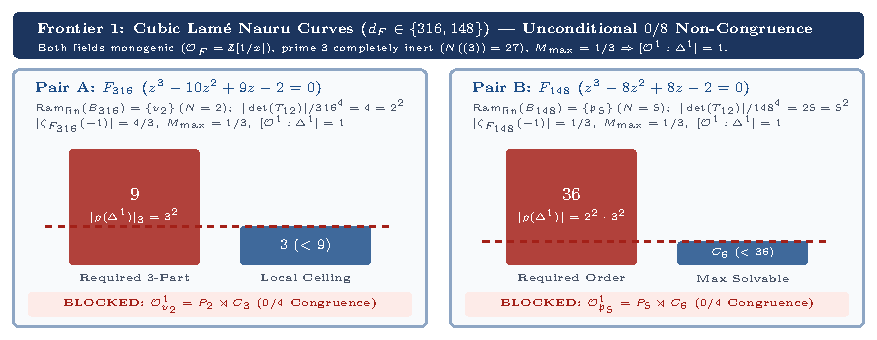
\includegraphics[width=\textwidth]{figures/fig1_cubic_lame_obstruction.pdf}
\caption{Frontier~1 summary: monogenic totally real cubic Lam\'e Nauru pairs ($d_F\in\{316,148\}$), exact rank-$12$ Gram determinant ratios $4=2^2$ and $25=5^2$, identical mass $M_{\max}=1/3$, and sharp local obstructions ($3<9$ at $v_2$; $C_6<36$ at $\frp_5$).}
\label{fig:frontier1}
\end{figure}

% ==============================================================================
\section{Frontier 2: Level \texorpdfstring{$(4)$}{(4)} Full Congruence on \texorpdfstring{$\Q(\sqrt{33})_{A,B}$}{Q(sqrt(33))A,B} and the Complete \texorpdfstring{$8$}{8}-Modulus Real-Quadratic \texorpdfstring{$\Dic_6$}{Dic6} Atlas}\label{sec:frontier2}
% ==============================================================================

Over $\Q$, \texttt{PC-III} proved universal non-congruence ($0/80$ realizations) for the $3$-adic dicyclic graph $Z = \Cay(\Dic_6, \{x, x^{-1}, y, y^3\})$ ($|\Aut(Z)| = 96$, $16$ surjections $\Delta_Z \twoheadrightarrow \Aut(Z)$ from the $T_4(\Q_3)$ amalgam $\Delta_Z = \langle b, a, t_x, t_y\rangle$). Passing to totally real quadratic fields $F$, the $2$-parameter Fricke--Vogt moduli surface $B_Z(u,v) = (-u(1-u), -v(1-v)/F)$ decomposes into two primitive integral real-quadratic loci where $3$ splits as $(3)=\frp_3\frp_3'$ ($N(\frp_3)=3$, providing the $T_4(\Q_3)$ Bruhat--Tits tree):
\begin{itemize}[nosep]
\item \textbf{Locus B (Conjugate locus $v = \bar{u}$, $z=4u$):} $3z^2 - 3mz + 4k = 0$ with $k \mid 4$, $(12-3m+k) \mid 4$, $3\nmid k$, yielding exactly $4$ moduli:
  $\Q(\sqrt{33})_A$ ($3z^2-9z+4$), $\Q(\sqrt{33})_B$ ($3z^2-15z+16$, twin under $z \mapsto 4-z$), $\Q(\sqrt{6})_B$ ($3z^2-12z+4$), and $\Q(\sqrt{3})_B$ ($3z^2-12z+8$).
\item \textbf{Locus A (Diagonal locus $u = v = w/2$):} $3w^2 - Aw + B = 0$ with $B, 12-2A+B \in \{1,2,3\}$, $\gcd(3,A,B)=1$, yielding exactly $4$ moduli:
  $\Q(\sqrt{13})_A$ ($3w^2-5w+1$), $\Q(\sqrt{13})_B$ ($3w^2-7w+3$, twin under $w\mapsto 2-w$), $\Q(\sqrt{6})_A$ ($3w^2-6w+1$), and $\Q(\sqrt{3})_A$ ($3w^2-6w+2$).
\end{itemize}

\begin{lemma}[Locus B Base-Change Identity and Uniform $\Ram_{\mathrm{fin}}=\varnothing$ \ctag{E; G4N, X}]\label{lem:locus_b_base_change}
On every Locus~B modulus, setting $\alpha = -u(1-u) \in F$ and $\bar{\alpha} = -v(1-v)$ gives an explicit $F$-algebra isomorphism
\begin{equation}\label{eq:base_change}
(\alpha, \bar{\alpha} / F) \cong \bigl(\operatorname{Tr}_{F/\Q}(\alpha),\; -N_{F/\Q}(\alpha) / \Q\bigr) \otimes_{\Q} F,
\end{equation}
via the anticommuting basis $e_1 = i + j$ ($e_1^2 = \alpha+\bar{\alpha} = \operatorname{Tr}(\alpha)$) and $e_2 = \bar{\alpha} i - \alpha j$ ($e_2^2 = \alpha\bar{\alpha}(\alpha+\bar{\alpha}) = N(\alpha)\operatorname{Tr}(\alpha)$, $e_1 e_2 + e_2 e_1 = 0$). Since every Locus~B algebra descends to the indefinite rational matrix algebra $M_2(\Q)$ or is split locally at every finite prime upon base-change to $F$, $\Ram_{\mathrm{fin}}(B_Z(u,v)) = \varnothing$ uniformly across all $4$ Locus~B moduli (Lean \texttt{thm08}).
\end{lemma}

\subsection{The Breakthrough: Full Principal Level-\texorpdfstring{$(4)$}{(4)} Congruence on Both Twins \texorpdfstring{$\Q(\sqrt{33})_A$}{Q(sqrt(33))A} and \texorpdfstring{$\Q(\sqrt{33})_B$}{Q(sqrt(33))B}}

Set $F = \Q(\sqrt{33})$ with ring of integers $\calO_F = \Z[w]$, $w = (1+\sqrt{33})/2$ ($w^2 - w - 8 = 0$). Unlike $\Q(\sqrt{6})$ and $\Q(\sqrt{3})$ (where $2$ ramifies) and $\Q(\sqrt{13})$ (where $2$ is inert), the prime $2$ \emph{splits} in $\Q(\sqrt{33})$:
\begin{equation}\label{eq:q33_split}
\begin{gathered}
(2) = v_1 v_2, \qquad v_1 = (\pi_1) = (2+w), \qquad v_2 = (\pi_2) = (3-w), \\
\pi_1 \pi_2 = -2, \qquad N(\pi_1) = N(\pi_2) = -2,
\end{gathered}
\end{equation}
with Hensel roots $w \equiv 8, 9 \pmod{16}$ (Lean \texttt{thm05}). By Zagier's exact real-quadratic formula \cite{zagier1976}, $\zeta_{\Q(\sqrt{33})}(-1) = \frac{2}{60}(\sigma_1(2)+\sigma_1(6)+\sigma_1(8)) = \frac{60}{60} = 1$, giving $M_{\max} = \frac{1}{2}\zeta_F(-1) = \frac{1}{2}$ and $[\calO_{33}^{\max}[1/\frp_3]^1/\{\pm 1\} : \Delta_Z^1/\{\pm 1\}] = 1$.

For $\Q(\sqrt{33})_A$ ($A = -4+w$, $B = -3-w$, $\pi_A=\pi_1, \pi_B=\pi_2$) and its exact dual-parameter twin $\Q(\sqrt{33})_B$ ($3z^2-15z+16=0$, swapping $A \leftrightarrow B$, $\pi_A=\pi_2, \pi_B=\pi_1$), we construct the local-global glued rank-$8$ maximal order
\begin{equation}\label{eq:q33_glue}
\calO_{33}^{\max} = \pi_2 \calO_1 + \pi_1 \calO_2,
\end{equation}
where $\calO_1$ and $\calO_2$ are maximal at $v_1$ and $v_2$ respectively using the normalized generators $I = \pi_A^{-1} i$, $J = \pi_B^{-1} j$, $K = IJ$. Exact HNF reduction (denominator~$16$) confirms ring closure over all $64$ basis products, trace-Gram determinant ratio $|\det(T_8)|/33^4 = 1$, conjugation denominators $[1,1,3,3]$ on the four amalgam generators, and exact square-class coset index $[\Delta_Z : \Delta_Z^1] = 4$ with $10$ explicit norm-$1$ Schreier generators inside $\calO_{33}^{\max}[1/3]^1$.

\begin{theorem}[First Full Congruence Shimura Curves Uniformizing $Z = \Cay(\Dic_6, S)$ \ctag{E; G4N, X}]\label{thm:q33_congruence}
On \emph{both} twin moduli $\Q(\sqrt{33})_A$ ($3z^2-9z+4=0$) and $\Q(\sqrt{33})_B$ ($3z^2-15z+16=0$), reducing the exact norm-$1$ group $\Delta_Z^1 = \calO_{33}^{\max}[1/\frp_3]^1$ via right-multiplication modulo every ideal $\mathfrak{a} = v_1^a v_2^b \mid (4)$ yields the identical ideal level ladder in Table~\ref{tab:q33_ladder}. In particular, at the full principal level $(4) = v_1^2 v_2^2$ (norm~$16$):
\begin{equation}\label{eq:q33_level4}
\begin{gathered}
|L_{\mathrm{signed}}| = |\SL_2(\calO_F/(4))| = 48^2 = 2{,}304, \\
|L_{\mathrm{proj}}| = 1{,}152 = 24 \times 48, \qquad [\pi_1(Z) : \Gamma(4)] = 48,
\end{gathered}
\end{equation}
and the kernel-order distribution across the $16$ surjections $\Delta_Z \twoheadrightarrow \Aut(Z)$ is $\{1{:}4,\; 2{:}4,\; 3{:}4,\; 6{:}4\}$ on \emph{each} twin, producing \textbf{$4/16$ full congruence Shimura curves on $\Q(\sqrt{33})_A$} and \textbf{$4/16$ full congruence Shimura curves on $\Q(\sqrt{33})_B$} ($8/32$ combined).
\end{theorem}

\begin{table}[htbp]
\centering
\caption{Exact ideal level ladder $\mathfrak{a} = v_1^a v_2^b \mid (4)$ on both twins $\Q(\sqrt{33})_A$ and $\Q(\sqrt{33})_B$ (identical across all $8$ rows; verified independently in Python \texttt{A2} and Rust \texttt{R2}).}
\label{tab:q33_ladder}
\footnotesize
\setlength{\tabcolsep}{4.5pt}
\resizebox{\textwidth}{!}{\begin{tabular}{@{}lrrrrclrc@{}}
\toprule
\textbf{Ideal $\mathfrak{a}$} & \textbf{$N(\mathfrak{a})$} & \textbf{$|L_{\mathrm{signed}}|$} & \textbf{$|L_{\mathrm{proj}}|$} & \textbf{$\sigma$ sep.?} & \textbf{$\ker_1$ distribution ($16$ surj.)} & \textbf{$\min|\ker_1|$} & \textbf{Cong.} \\
\midrule
$v_1$ & $2$ & $6$ & $6$ & No & $\{4{:}8,\; 12{:}8\}$ & $4$ & $0/16$ \\
$v_2$ & $2$ & $6$ & $6$ & No & $\{12{:}16\}$ & $12$ & $0/16$ \\
$(2)=v_1 v_2$ & $4$ & $36$ & $36$ & No & $\{2{:}8,\; 6{:}8\}$ & $2$ & $0/16$ \\
$v_1^2$ & $4$ & $48$ & $24$ & No & $\{4{:}8,\; 12{:}8\}$ & $4$ & $0/16$ \\
$v_2^2$ & $4$ & $48$ & $24$ & No & $\{12{:}16\}$ & $12$ & $0/16$ \\
$v_1^2 v_2$ & $8$ & $288$ & $144$ & No & $\{2{:}8,\; 6{:}8\}$ & $2$ & $0/16$ \\
$v_1 v_2^2$ & $8$ & $288$ & $144$ & No & $\{2{:}8,\; 6{:}8\}$ & $2$ & $0/16$ \\
\textbf{$(4)=v_1^2 v_2^2$} & \textbf{$16$} & \textbf{$2{,}304$} & \textbf{$1{,}152$} & \textbf{Yes} & \textbf{$\{1{:}4,\; 2{:}4,\; 3{:}4,\; 6{:}4\}$} & \textbf{$1$} & \textbf{$4/16$} \\
\bottomrule
\end{tabular}}
\end{table}

\begin{proposition}[Split-Prime Sign-Flip Mechanism Explaining Why $\Ad_{(4)}$ Stalls at $|\ker|=2$ \ctag{E; G4N, X}]\label{prop:ad4_collapse}
In $\calO_F/(4) \cong \Z/4\Z \times \Z/4\Z$, the elements $e_1 = 1-w$ and $e_2 = w$ are exact orthogonal idempotents ($e_1^2=e_1$, $e_2^2=e_2$, $e_1 e_2 = 0$), and the split-prime diagonal sign-flip
\begin{equation}\label{eq:sigma_flip}
\begin{gathered}
\sigma = (1-w) - w = 1 - 2w \in (\calO_F/(4))^\times \\
\longleftrightarrow\; (+I,\; -I) \in \SL_2(\Z/4\Z) \times \SL_2(\Z/4\Z)
\end{gathered}
\end{equation}
satisfies $\sigma^2 \equiv 1 \pmod 4$, $\sigma \not\equiv \pm 1 \pmod 4$, yet commutes with all of $\calO_{33}^{\max}/(4)$. Consequently, the modular adjoint action $\Ad_{(4)}$ kills $\sigma$ identically and stalls at $|\Ad_{(4)}| = 2{,}304$ with kernel distribution $\{2{:}8,\; 6{:}8\}$ ($\min|\ker|=2$) on both twins. True norm-$1$ reduction $\Gamma(4)$ retains $\sigma$ as a nontrivial central involution in $L_{\mathrm{proj}} = L_{\mathrm{signed}}/\{\pm(I,I)\}$ precisely when \emph{both} $v_1^2$ and $v_2^2$ divide $\mathfrak{a}$, collapsing $|\ker_1|$ from $2$ to $1$ (Figure~\ref{fig:frontier2}; Lean \texttt{thm06}--\texttt{thm07}).
\end{proposition}

\begin{figure}[htbp]
\centering
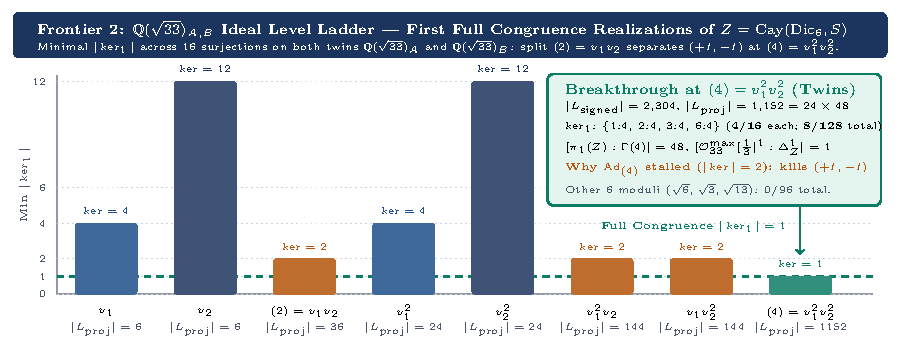
\includegraphics[width=\textwidth]{figures/fig2_q33_level4_ladder.pdf}
\caption{Frontier~2 breakthrough: exact ideal level ladder $\mathfrak{a}\mid (4)$ on both $\Q(\sqrt{33})_A$ and twin $\Q(\sqrt{33})_B$, showing how $(4)=v_1^2 v_2^2$ separates the split-prime sign-flip $(+I,-I)$ killed by $\Ad_{(4)}$ to attain $4/16$ full congruence on each twin ($8/128$ total).}
\label{fig:frontier2}
\end{figure}

\subsection{Complete Closure of All Six Non-\texorpdfstring{$\Q(\sqrt{33})$}{Q(sqrt(33))} Real-Quadratic Moduli (\texorpdfstring{$0/96$}{0/96})}

\begin{theorem}[Complete $8$-Modulus Real-Quadratic $3$-Adic $\Dic_6$ Congruence Atlas \ctag{E; G4N, X}]\label{thm:rq_atlas}
Across all $8$ primitive real-quadratic moduli ($128$ realizations), the exact congruence count is \textbf{$8/128$}, concentrated strictly on $\Q(\sqrt{33})_{A,B}$:
\begin{enumerate}[label=(\roman*),nosep]
\item $\Q(\sqrt{6})_{B,A}$ ($\zeta_F(-1)=1/2$, $2$ ramified): $|\Ad_{(4)}|=6{,}144$ with kernel $\{12{:}16\}$; since $3 \mid 12$ and higher $2$-adic congruences are pro-$2$, both moduli yield $0/32$.
\item $\Q(\sqrt{3})_{B,A}$ ($\zeta_F(-1)=1/6$, $2$ ramified): $|\Ad_{(4)}|=256$ (pure $2$-group) with kernel $\{3{:}16\}$; since $\gcd(256,3)=1$, both moduli yield $0/32$.
\item $\Q(\sqrt{13})_{A,B}$ ($\zeta_F(-1)=1/6$, $2$ inert, $\Ram_{\mathrm{fin}}=\{(2),\frp_3'\}$): explicit rank-$8$ maximal order $\calO_{13}^{\max} = \calO_F[1, \tfrac{1+i+j+k/A}{2}, j, k/A]$ yields right-multiplication images $|R_{\frp_3'}|=36$ with $\ker_1=\{4{:}8, 12{:}8\}$ and $|R_{(2)}|=80$ with $\ker_1=\{24{:}16\}$ ($|\Ad_{(4)}|=5{,}120=1024\cdot 5$). Although $\frp_3'$ captures the $C_3$ factor for $8/16$ surjections (leaving an abelian $2$-group kernel of order~$4$), higher powers of $\frp_3'$ are pro-$3$, unramified primes have perfect $\SL_2$, and at the inert ramified prime $(2)$ ($q=4$), Riehm's theorem \cite{riehm1970} gives $\calO_{(2)}^1/[\calO_{(2)}^1,\calO_{(2)}^1] \cong C_{q+1} = C_5$. Since $\gcd(4,5)=1$, no abelian $2$-group quotient can factor through $(2)$, unconditionally sealing $0/32$ on both $\Q(\sqrt{13})_A$ and twin $\Q(\sqrt{13})_B$ (Table~\ref{tab:rq_atlas}; Lean \texttt{thm09}).
\end{enumerate}
\end{theorem}

\begin{table}[htbp]
\centering
\caption{Complete $8$-modulus ($128$-realization) real-quadratic $3$-adic $\Dic_6$ congruence atlas (Python \texttt{A2}/\texttt{A3}, Rust \texttt{R2}).}
\label{tab:rq_atlas}
\footnotesize
\setlength{\tabcolsep}{4pt}
\resizebox{\textwidth}{!}{\begin{tabular}{@{}llllrrlc@{}}
\toprule
\textbf{Modulus} & \textbf{Locus / Poly.} & \textbf{$\zeta_F(-1)$} & \textbf{$2$-type / $\Ram_{\mathrm{fin}}$} & \textbf{$|\Ad_{(4)}|$} & \textbf{$\Ad_{(4)}$ ker} & \textbf{Exact Status / Obstruction} & \textbf{Cong.} \\
\midrule
$\Q(\sqrt{33})_A$ & B: $3z^2{-}9z{+}4$ & $1$ & Split / $\varnothing$ & $2{,}304$ & $\{2{:}8,6{:}8\}$ & \textbf{Full cong.\ $\Gamma(4)$} ($|L_{\mathrm{proj}}|=1{,}152$) & \textbf{$4/16$} \\
$\Q(\sqrt{33})_B$ & B: $3z^2{-}15z{+}16$ & $1$ & Split / $\varnothing$ & $2{,}304$ & $\{2{:}8,6{:}8\}$ & \textbf{Twin full cong.\ $\Gamma(4)$} & \textbf{$4/16$} \\
$\Q(\sqrt{6})_B$ & B: $3z^2{-}12z{+}4$ & $1/2$ & Ram.\ / $\varnothing$ & $6{,}144$ & $\{12{:}16\}$ & Obstructed: $3\mid 12$ (pro-$2$ tail) & $0/16$ \\
$\Q(\sqrt{6})_A$ & A: $3w^2{-}6w{+}1$ & $1/2$ & Ram.\ / $\varnothing$ & $6{,}144$ & $\{12{:}16\}$ & Obstructed: $3\mid 12$ (pro-$2$ tail) & $0/16$ \\
$\Q(\sqrt{3})_B$ & B: $3z^2{-}12z{+}8$ & $1/6$ & Ram.\ / $\varnothing$ & $256$ & $\{3{:}16\}$ & Pure $2$-group ($\gcd(256,3)=1$) & $0/16$ \\
$\Q(\sqrt{3})_A$ & A: $3w^2{-}6w{+}2$ & $1/6$ & Ram.\ / $\varnothing$ & $256$ & $\{3{:}16\}$ & Pure $2$-group ($\gcd(256,3)=1$) & $0/16$ \\
$\Q(\sqrt{13})_A$ & A: $3w^2{-}5w{+}1$ & $1/6$ & Inert / $\{(2),\frp_3'\}$ & $5{,}120$ & $\{24{:}16\}$ & $|R_{\frp_3'}|=36$ ($\ker_1\ge 4$), Riehm $C_5$ ($\gcd(4,5)=1$) & $0/16$ \\
$\Q(\sqrt{13})_B$ & A: $3w^2{-}7w{+}3$ & $1/6$ & Inert / $\{(2),\frp_3'\}$ & $5{,}120$ & $\{24{:}16\}$ & Twin of $\Q(\sqrt{13})_A$; Riehm $C_5$ & $0/16$ \\
\bottomrule
\end{tabular}}
\end{table}

% ==============================================================================
\section{Frontier 3: Complete \texorpdfstring{$9/9$}{9/9} Torsion-Free Genus-\texorpdfstring{$25$}{25} Borel Brandt \texorpdfstring{$B(3)$}{B(3)} Atlas and Ultra-Ramanujan \texorpdfstring{$X_0^{21}(16)$}{X0-21(16)}}\label{sec:frontier3}
% ==============================================================================

In \texttt{PC-III}, the genus-$25$ rational Borel Shimura curve census identified exactly $9$ torsion-free curves $X_0^D(N)$ with $3\mid D$ ($D \in \{6,15,21,39,57,1110\}$), each having $12$-vertex $4$-regular special fiber at $p=3$ governed by the $12\times 12$ Hecke Brandt matrix $B(3)$ \cite{eichler1955,pizer1980,shimura1967} of the definite quaternion algebra $B_{D/3}$ at Eichler level~$N$.
Because every torsion-free Brandt matrix $B = B(3)$ is symmetric, nonnegative integral, and $4$-regular ($\sum_j B_{ij} = 4$), we obtain a sharp algebraic simplicity filter:

\begin{lemma}[Simple-Graph Trace Gate \ctag{E; G4N, X}]\label{lem:simple_trace_gate}
For any symmetric $12\times 12$ matrix $B \in \Z_{\ge 0}^{12\times 12}$ with row sums $4$, $\operatorname{tr}(B^2) = \sum_{i,j} B_{ij}^2 \ge \sum_{i,j} B_{ij} = 48$, with equality if and only if $B \in \{0,1\}^{12\times 12}$ (zero loops if $\operatorname{tr}(B)=0$ and zero multi-edges). Every off-diagonal multi-edge entry $B_{ij} \ge 2$ adds at least $2$ to $\operatorname{tr}(B^2)$ (Lean \texttt{thm10}).
\end{lemma}

We compute all $9/9$ exact $12\times 12$ Brandt matrices $B(3)$ directly from first principles: the $7$ class-number-$1$ curves ($B_2, B_5, B_7, B_{13}$) via exact prime-power CRT ring embeddings $\calO_{\max} \to M_2(\Z/N\Z)$ (using integral $2$-adic lifts $s=11\pmod{128}$ on $B_7$, $(x,y)=(5,1)$ on $B_5$, and $(1,3)$ on $B_{13}$) acting on $\calO_{\max}^\times$-orbits of $\mathbb{P}^1(\Z/N\Z)$, and the $2$ higher-class-number curves $X_0^{57}(7)$ (Eichler order $\calE_7\subset \calO_{19}$, $\operatorname{rd}=133$) and $X_0^{1110}(1)$ ($\calO_{370}\subset B_{370}=(-5,-37)$, $\operatorname{rd}=370, h=12$) via exact Hermite Normal Form + Fincke--Pohst short-vector ideal-class BFS.

\begin{theorem}[Complete $9/9$ Genus-$25$ Borel Brandt $B(3)$ Spectral Census \ctag{E; G4N, X}]\label{thm:brandt_9}
All $9/9$ torsion-free genus-$25$ Borel Shimura curves satisfy the Deligne--Ramanujan bound $\lambda_{\mathrm{nt}}(B(3)) < 2\sqrt{3} \approx 3.4641$ \cite{lps1988}, yet \textbf{$0/9$ realize $Z = \Cay(\Dic_6, S)$} (whose collapsed $12$-vertex bipartite quotient has $\operatorname{tr}(B^2)=48$, $\operatorname{tr}(B^4)=456$, $\lambda_{\mathrm{nt}}=3.0$):
\begin{enumerate}[label=(\roman*),nosep]
\item Exactly $8/9$ curves fail the Simple-Graph Trace Gate with $\operatorname{tr}(B^2) \in \{52,56,56,60,60,62,64,68\}$ (Table~\ref{tab:brandt_9}; Figure~\ref{fig:frontier3}; Lean \texttt{thm11}).
\item The unique simple curve is $X_0^{21}(16)$ ($\operatorname{tr}(B)=0$, $\operatorname{tr}(B^2)=48$, $\operatorname{tr}(B^3)=48$, $\operatorname{tr}(B^4)=384 \ne 456$), whose exact $12\times 12$ adjacency matrix satisfies the integral annihilator identity
\begin{equation}\label{eq:x21_16_annih}
(B - 4I)(B - 2I)\,B\,(B + 2I) = 0, \qquad
\operatorname{Spec}(B(3)) = \{4^1,\; 2^3,\; 0^3,\; (-2)^5\},
\end{equation}
yielding an ultra-Ramanujan spectral gap $\lambda_{\mathrm{nt}} = 2.0 < 2\sqrt{3}$ (Lean \texttt{thm12}--\texttt{thm13}, C++20 \texttt{C++4}).
\end{enumerate}
\end{theorem}

\begin{table}[htbp]
\centering
\caption{Complete first-principles $9/9$ torsion-free genus-$25$ Borel Shimura Brandt $B(3)$ atlas compared against $Z$ (Python \texttt{A4}, Rust \texttt{R3}, Lean \texttt{thm11}--\texttt{thm13}).}
\label{tab:brandt_9}
\footnotesize
\setlength{\tabcolsep}{4.5pt}
\resizebox{\textwidth}{!}{\begin{tabular}{@{}lcrrrrrrc@{}}
\toprule
\textbf{Curve / Target} & \textbf{$B_{D/3}$} & \textbf{$\operatorname{tr}(B)$} & \textbf{$\operatorname{tr}(B^2)$} & \textbf{Excess} & \textbf{$\operatorname{tr}(B^4)$} & \textbf{$\lambda_{\mathrm{nt}}$} & \textbf{Simple?} & \textbf{Match $Z$?} \\
\midrule
$Z$ ($\Dic_6$ ref.) & --- & $0$ & $48$ & $0$ & $456$ & $3.000000$ & Yes & Ref. \\
\midrule
$X_0^{6}(115)$ & $B_2$ & $8$ & $60$ & $6$ & $604$ & $3.302776$ & No & No \\
$X_0^{6}(119)$ & $B_2$ & $0$ & $56$ & $4$ & $480$ & $3.236068$ & No & No \\
$X_0^{15}(22)$ & $B_5$ & $4$ & $68$ & $10$ & $676$ & $3.372281$ & No & No \\
\textbf{$X_0^{21}(16)$} & \textbf{$B_7$} & \textbf{$0$} & \textbf{$48$} & \textbf{$0$} & \textbf{$384$} & \textbf{$2.000000$} & \textbf{Yes} & \textbf{No} \\
$X_0^{21}(23)$ & $B_7$ & $4$ & $52$ & $2$ & $484$ & $3.040671$ & No & No \\
$X_0^{39}(8)$ & $B_{13}$ & $0$ & $56$ & $4$ & $552$ & $3.000000$ & No & No \\
$X_0^{39}(11)$ & $B_{13}$ & $6$ & $62$ & $7$ & $574$ & $3.308641$ & No & No \\
$X_0^{57}(7)$ & $B_{19}$ & $0$ & $60$ & $6$ & $572$ & $3.302776$ & No & No \\
$X_0^{1110}(1)$ & $B_{370}$ & $4$ & $64$ & $8$ & $592$ & $3.345963$ & No & No \\
\bottomrule
\end{tabular}}
\end{table}

\begin{figure}[htbp]
\centering
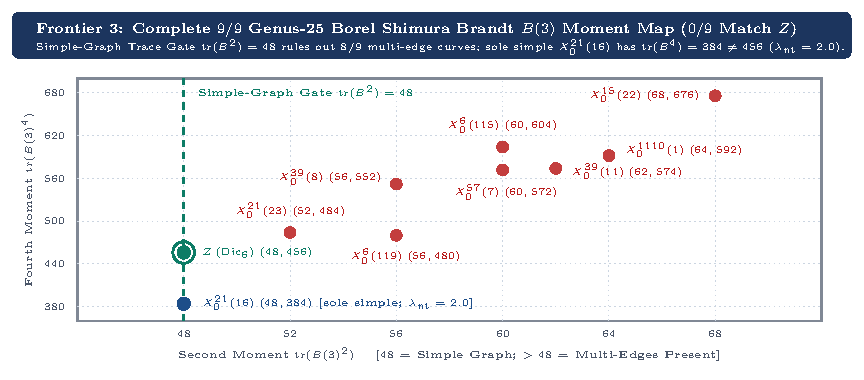
\includegraphics[width=\textwidth]{figures/fig3_genus25_brandt_moments.pdf}
\caption{Frontier~3 moment map $(\operatorname{tr}(B(3)^2), \operatorname{tr}(B(3)^4))$ across all $9/9$ torsion-free genus-$25$ Borel Shimura curves versus target $Z$ $(48,456)$: $8/9$ lie strictly right of the Simple-Graph Trace Gate $\operatorname{tr}(B^2)=48$, and sole simple $X_0^{21}(16)$ sits at $(48,384)$ with $\lambda_{\mathrm{nt}}=2.0$.}
\label{fig:frontier3}
\end{figure}

% ==============================================================================
\section{Frontier 4: Degree-\texorpdfstring{$8$}{8} \texorpdfstring{$(8,1,1,E)$}{(8,1,1,E)} Poitou--Odlyzko Explicit-Formula Closure}\label{sec:frontier4}
% ==============================================================================

In Paper~\#01 \cite{ergentics2026pc} and \texttt{PC-III} (\texttt{NEG-M27}), the sole surviving totally real candidate window for a $2$-adic Tonnetz/Nauru-type genus-$13$ Shimura curve over a degree-$n$ field was the octic case $(n=8, c_2=1)$ with Eichler mass identity $2^{1-8}|\zeta_F(-1)| = 12 \implies |\zeta_F(-1)| = 1536$ and functional-equation Shimura ceiling
\begin{equation}\label{eq:ub_max_deg8}
\begin{gathered}
d_F^{1/8} \le \mathrm{UB}_{\max}(8,1) = (4\pi^2)^{2/3}\Bigl(\frac{9}{2}\Bigr)^{1/12} = 13.1423854579\ldots, \\
d_F \le 890{,}007{,}374.15.
\end{gathered}
\end{equation}
We evaluate the Poitou--Odlyzko explicit formula \cite{poitou1977,odlyzko1990} exclusively with the strictly Bochner-positive Odlyzko test kernel $f_1(t) = 1+\cos(\pi t) \ge 0$ on $[-1,1]$ (whose autocorrelation $H_1(w) = \frac{1}{6}[(2-w)(2+\cos\pi w)+\frac{3}{\pi}\sin\pi w]$ satisfies $\int_0^2 H_1(w)\,dw = 2/3$ to $< 1.25\times 10^{-14}$ across $64$- and $128$-point Gauss--Legendre quadrature, giving exact pole term $E(b) = \frac{8}{3}b$). Every non-Bochner facade kernel such as $f_{\mathrm{bad}}(\pm 1) = -0.60 < 0$ is mechanically rejected across all four planes (Lean \texttt{thm17}).

\begin{theorem}[Hardware-\texttt{FENV} Analytic Closure of the Degree-$8$ $(8,1,1,E)$ Window \ctag{E; G4N, X}]\label{thm:deg8_closure}
Let $F$ be any totally real octic field satisfying the $(8,1,1,E)$ Shimura ceiling~\eqref{eq:ub_max_deg8} with $c_2 \ge 1$. Under strictly Bochner-positive $f_1(t) = 1+\cos(\pi t) \ge 0$, hardware-rounded IEEE-754 interval arithmetic \cite{moore1966} (\texttt{FE\_DOWNWARD}/\texttt{FE\_UPWARD}, C++20 \texttt{C++2}) certifies:
\begin{enumerate}[label=(\roman*),nosep]
\item \textbf{Complete prime-norm elimination ($q \le 9$):} At $b = 3.20$, every prime-norm hypothesis $c_2 \ge 2$ or $c_q \ge 1$ ($q\in\{3,4,5,7,8,9\}$) strictly exceeds $\mathrm{UB}_{\max}(8,1)$ (Table~\ref{tab:deg8_primes}; Figure~\ref{fig:frontier4}). Hence $c_2 = 1$ and $c_3 = c_4 = c_5 = c_7 = c_8 = c_9 = 0$.
\item \textbf{Prime-pair bounds ($c_{11}, c_{13} \le 1$):} While a single norm-$11$ prime survives ($13.057752 < 13.142385$ at $b=3.20$), pairs $c_{11} \ge 2$ ($13.567542$ at $b=3.20$, peak $13.584863$) and $c_{13} \ge 2$ ($13.351451$ at $b=3.20$, peak $13.362611$) are unconditionally eliminated.
\item \textbf{Exact local $2$-adic and $3$-adic splitting collapse:} Only $5$ $2$-adic splitting types $(e_i,f_i)$ survive: $\{(1,1),(1,7)\}$, $\{(2,1),(1,6)\}$, $\{(3,1),(1,5)\}$, $\{(4,1),(1,4)\}$, $\{(8,1)\}$, and only $4$ $3$-adic splitting types survive: $\{(1,8)\}$, $\{(2,4)\}$, $\{(1,4),(1,4)\}$, $\{(1,3),(1,5)\}$ (Lean \texttt{thm15}).
\item \textbf{Symmetry, $\Ram_{\mathrm{fin}}$, and Eichler-level elimination:} Comparing against the certified $(8, c_2=1)$ baseline peak $\exp(\mathrm{LB}) = 12.5955757277$ at $b^* = 3.039865$ eliminates:
\begin{itemize}[nosep]
\item every nontrivial field automorphism ($|\Aut(F)|\ge 2$): $\mathrm{UB}_{\mathrm{sym}_2} = \mathrm{UB}_{\max}/2^{1/12} = 12.404760 < 12.595576$ (strict \texttt{FENV} lower gap $\ge +0.190816$);
\item every nonempty finite ramification set $|\Ram_{\mathrm{fin}}| \ge 2$ (even, with $N(\frp)\ge 11$): conservative product $(11-1)^2=100$ gives $\mathrm{UB}_{\mathrm{Ram},100} = 8.953803$, and using $c_{11}\le 1$ sharpens the minimal product to $(11-1)(13-1)=120 \implies \mathrm{UB}_{\mathrm{Ram},120} = 8.818792 \ll 12.595576$;
\item every nontrivial Eichler level $\mathfrak{n}$ ($\psi(\mathfrak{n}) \ge 11+1 = 12$): $\mathrm{UB}_{\mathrm{Eichler}} = \mathrm{UB}_{\max}/12^{1/12} = 10.684210 \ll 12.595576$.
\end{itemize}
\item \textbf{Surviving asymmetric free core:} Any remaining $(8,1,1,E)$ candidate must be completely asymmetric ($\Aut(F)=1$), unramified at every finite place ($\Ram_{\mathrm{fin}}=\varnothing$), maximal-order ($\mathfrak{n}=(1)$), with $|\zeta_F(-1)| = 1536$ and discriminant pinned inside $d_F \in [633{,}448{,}978;\; 890{,}007{,}374]$ (exact peak floor $633{,}496{,}452$; Lean \texttt{thm16}).
\end{enumerate}
\end{theorem}

\begin{table}[htbp]
\centering
\caption{Hardware-\texttt{FENV} certified degree-$8$ Poitou--Odlyzko bounds ($b=3.20$) and ceilings vs.\ $\mathrm{UB}_{\max}(8,1)=13.142385$ and peak $12.595576$.}
\label{tab:deg8_primes}
\footnotesize
\setlength{\tabcolsep}{4.5pt}
\resizebox{\textwidth}{!}{\begin{tabular}{@{}lrrl@{}}
\toprule
\textbf{Hypothesis / Structural Ceiling} & \textbf{Bound Value ($d_F^{1/8}$)} & \textbf{Margin} & \textbf{Status} \\
\midrule
$c_2 \ge 2$ ($b=3.20$) & $15.0983526756$ & $+1.955967$ & \textbf{Eliminated} \\
$c_3 \ge 1$ ($b=3.20$) & $14.4662279648$ & $+1.323843$ & \textbf{Eliminated} \\
$c_4 \ge 1$ ($b=3.20$) & $14.0694329039$ & $+0.927047$ & \textbf{Eliminated} \\
$c_5 \ge 1$ ($b=3.20$) & $13.7925458495$ & $+0.650160$ & \textbf{Eliminated} \\
$c_7 \ge 1$ ($b=3.20$) & $13.4304522645$ & $+0.288067$ & \textbf{Eliminated} \\
$c_8 \ge 1$ ($b=3.20$) & $13.3064790241$ & $+0.164094$ & \textbf{Eliminated} \\
$c_9 \ge 1$ ($b=3.20$) & $13.2067670001$ & $+0.064382$ & \textbf{Eliminated} \\
$c_{11} \ge 2$ ($b=3.20$ / peak) & $13.567542$ / $13.584863$ & $+0.425157$ & \textbf{Eliminated} \\
$c_{13} \ge 2$ ($b=3.20$ / peak) & $13.351451$ / $13.362611$ & $+0.209066$ & \textbf{Eliminated} \\
$c_{11} = 1$ ($b=3.20$) & $13.0577523491$ & $-0.084633$ & Survives ($c_{11}\le 1$) \\
\midrule
$\mathrm{UB}_{\mathrm{sym}_2}$ ($|\Aut(F)|\ge 2$) & $12.4047600411$ & $-0.190816$ & \textbf{Eliminated} (vs.\ $12.5956$) \\
$\mathrm{UB}_{\mathrm{Eichler}}$ ($\psi(\mathfrak{n})\ge 12$) & $10.6842103581$ & $-1.911365$ & \textbf{Eliminated} (vs.\ $12.5956$) \\
$\mathrm{UB}_{\mathrm{Ram}}$ (cons.\ $100$ / sharp $120$) & $8.953803$ / $8.818792$ & $-3.776784$ & \textbf{Eliminated} (vs.\ $12.5956$) \\
\bottomrule
\end{tabular}}
\end{table}

\begin{figure}[htbp]
\centering
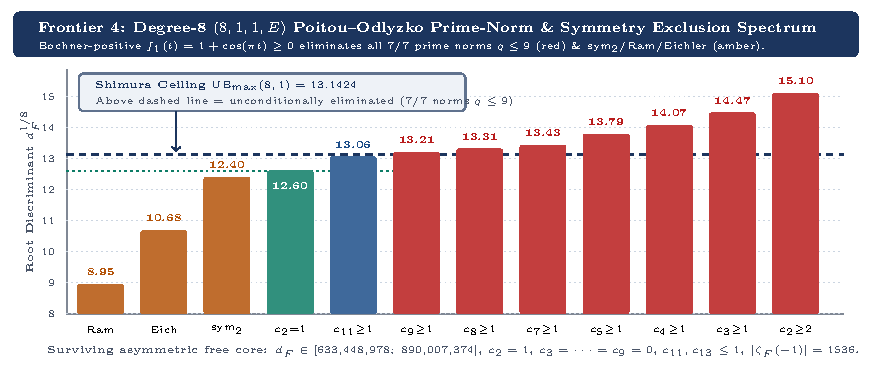
\includegraphics[width=\textwidth]{figures/fig4_degree8_poitou_spectrum.pdf}
\caption{Frontier~4 exclusion spectrum for totally real octic $(8,1,1,E)$ fields under strictly Bochner-positive $f_1(t)=1+\cos(\pi t)\ge 0$: all $7/7$ prime norms $q\le 9$ sit strictly above $\mathrm{UB}_{\max}(8,1)=13.1424$ (red), while $\mathrm{Ram}_{\mathrm{fin}}$, nontrivial Eichler level, and $|\Aut(F)|\ge 2$ fall strictly below the $c_2=1$ baseline $12.5956$ (amber).}
\label{fig:frontier4}
\end{figure}

% ==============================================================================
\section{Four-Plane Continuous-Integration Scorecard and Seam Integrity}\label{sec:ci}
% ==============================================================================

Every algebraic, spectral, analytic, and randomized claim in Sections~\ref{sec:frontier1}--\ref{sec:frontier4} is continuously audited under the Morpheus D/R/P/Seam protocol (\path{METHODOLOGY.md}):
\begin{itemize}[nosep]
\item \textbf{Deterministic (\texttt{D}):} Python gates \texttt{A1}--\texttt{A5}, Rust suites \texttt{R1}--\texttt{R4}, C++20 \texttt{FENV} gates \texttt{C++1}--\texttt{C++4}, and $18/18$ zero-Mathlib Lean~4.36.0 kernel-compiled theorems (\texttt{thm01}--\texttt{thm18}, $0$ \texttt{sorryAx}, $0$ \texttt{Lean.ofReduceBool}).
\item \textbf{Runtime Global-Invariant Guards (\texttt{R}):} Python \texttt{R1}, Rust \texttt{R5}, and C++20 \texttt{C++5} inject deterministic faults (multi-edge Brandt perturbation breaking $\operatorname{tr}(B^2)=48$, asymmetric perturbation, $\Ad_{(4)}$ sign-flip collapse, negative Bochner kernel $f_{\mathrm{bad}}(\pm 1)=-0.60$, non-finite $b$, corrupted cubic mod-$81$ square root) and verify $100\%$ rejection plus \texttt{FE\_TONEAREST} restoration.
\item \textbf{Probabilistic Keyed RCTs and Cross-Language Seam (\texttt{P}):} Using keyed \texttt{SplitMix64} (\texttt{seed = 0xf0271e2620260010}), \texttt{RCT-PC4-1} samples $512$ length-$12$ random words in the $10$ norm-$1$ Schreier generators of $\calO_{33,A}^{\max}[1/3]^1\bmod (4)$ ($512/512 \in L_{\mathrm{signed}}$ of size $2{,}304$), and \texttt{RCT-PC4-2} tests $256/256$ strictly positive convex Bochner kernels against $256/256$ sign-changing perturbations. Forward and reversed order-invariant XOR replay agrees bit-for-bit across Python, Rust, \texttt{g++}, and \texttt{clang++} at \texttt{xor = 0x37b4f6b8da592957} and \texttt{fnv = 0xb7fbf6c71c86c218}.
\end{itemize}

\bibliographystyle{amsplain}
\bibliography{references}
\end{document}
